\section{Luthfi Muhammad Nabil (1174035)}
\subsection{Data Geospasial}
Data Geospasial merupakan data yang isinya mengenai lokasi geografis, ukuran atau karakteristik obyek alam atau buatan manusia yang berada di lingkungan bumi baik di bawah permukaan, permukaan, atau atas permukaan. Objek yang dimaksud pada data geospasial salah satunya mencakup jalan, bangunan, gunung, laut, dan sebagainya. Untuk bentuk data geospasial sendiri berbentuk data vektor dan data gambar yang dibuat menjadi kumpulan data untuk aplikasi dapat memproses data tersebut. Selain data tersebut, informasi mengenai karakteristik obyek juga disimpan pada data geospasial seperti nama jalan, ukuran bangunan, nama tempat, dan lain sebagainya.
\break
Data Geospasial bersumber dari beberapa hal berikut : 
\begin{itemize}
	\item Rekaman Data Alat Permukaan : Untuk merekam data yang realtime, alat akan berperan pada pengiriman data geospasial. Alat yang dimaksud sepert Sensor pada Arduino.
	\item Satelit Luar Angkasa : Selain permukaan, data secara keseluruhan juga diperlukan untuk membuat data keseluruhan permukaan bumi dan data lainnya. 
	\item Data Pemerintah : Data yang sudah diukur oleh pemerintah sebelumnya juga akan dipakai untuk membuat karakteristik detail dari sebuah obyek. 
	\item Dan lain sebagainya.
\end{itemize}
Data geospasial sudah banyak digunakan pada banyak aplikasi. Data yang akan dipakai untuk menunjukan lokasi, tata letak daerah, dan sebagainya. Data geospasial juga memberi manfaat bagi yang menggunakan atau yang merasakan aplikasi yang memakai Data geospasial. Beberapa manfaat yang bisa didapat diantaranya : 
\begin{itemize}
	\item Dapat mencari sebuah tujuan hanya dengan menuliskan nama tempat atau alamat
	\item Mengetahui kondisi dari daerah berdasarkan data geospasial realtime yang dibuat oleh setempat
	\item Sebagai survey untuk beberapa lokasi yang perlu diperhatikan
	\item Sebagai pembelajaran mengenai geografis
\end{itemize}
\subsection{Link}
\subsection{Plagiarism}
\begin{figure}[H]
	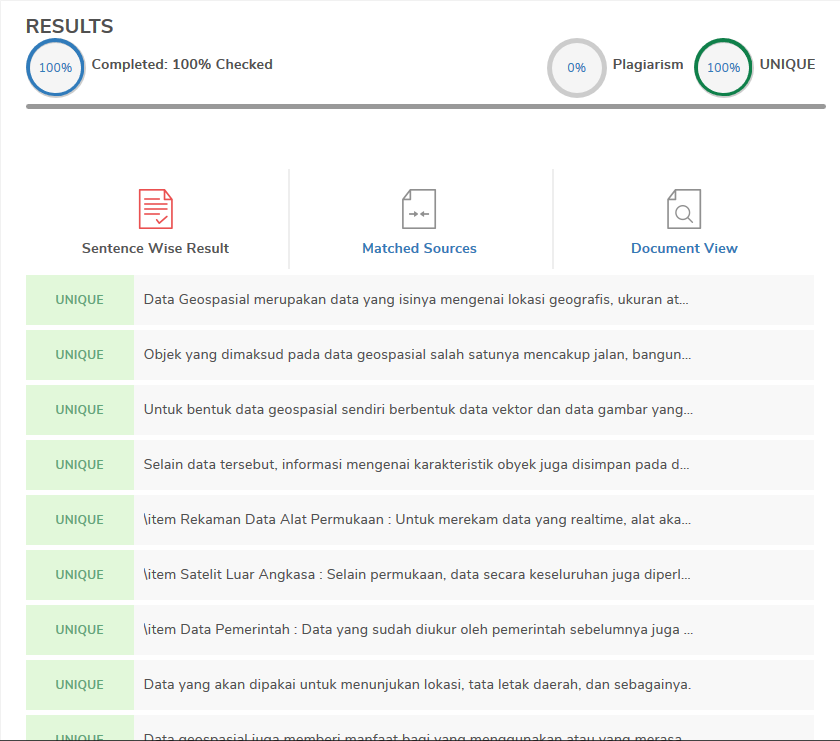
\includegraphics[width=10cm]{figures/1174035/tugas1/plagiat.png}
	\centering
	\caption{Hasil Pengecekan Plagiat}
\end{figure}

